\documentclass[11pt]{report}
\usepackage[a4paper, tmargin=2.54cm, bmargin=2.54cm, lmargin=3.17cm, rmargin=3.17cm]{geometry}
\newcommand{\head}[1]{\textnormal{\textbf{#1}}}

\usepackage{titlesec}   
\titleformat{\chapter}{\normalfont\huge\bf}{\thechapter}{20pt}{\huge\bf}


\author{authors}
\setcounter{tocdepth}{3}
\renewcommand{\figurename}{Figure}
\renewcommand{\listfigurename}{List of Figures}
\usepackage{graphicx}
\usepackage{booktabs}
\usepackage{natbib}
\usepackage[dvipsnames]{xcolor}
\usepackage{amssymb}
%\usepackage{helvet}

\usepackage{hyperref}	% Hyperlinks in document
\hypersetup{	% More info: https://www.sharelatex.com/learn/Hyperlinks
    colorlinks=true,
    citecolor = blue,	% References
    linkcolor=black,    % Table of contents
    filecolor=magenta,      
    urlcolor=cyan,
}

%MORE PACKAGES HERE
\usepackage{tikz}
\usepackage{blindtext}





\begin{document}

%%%%%%%%%%%%%%%%%%%%%%%%%%%%
%%%% FIRST PAGE
% Change the student's name
% thesis' title, and supervisors



\thispagestyle{empty}
\begin{titlepage}
   \noindent

 \begin{figure}[htb]
    \begin{minipage}[t]{.65\textwidth}
        Human-Centred AI Masters\\ 
	December \the\year\\
	THES H6011 Research Thesis, 30 Credits\\
    \end{minipage}
    \hfill
    \begin{minipage}[t]{.32\textwidth}
        
\includegraphics[width=\textwidth]{figures/hcaim-logo.png}
    \end{minipage}
    \hrule
   \end{figure}

	
	
	%Thesis title
	

\begin{center}
    {\LARGE\noindent \textbf{Predicting DublinBike Availability Using Spatio-Temporal Graph Convolutional Networks} \par}
	\vspace{0.5cm}
	
	%Author's name
	{\LARGE\noindent \emph{Saketh Reddy Chandupatla} \par}  

 \vspace{1cm}
 
\includegraphics[width=90mm]{figures/TUDublin_Colour_RGB.png}
     
\vspace{0.5cm}
   
 \vspace{0.5cm}
 {A thesis submitted in the partial fulfilment for the 

\textbf{Masters in Science  in Human-Centred Artificial Intelligence} \par}
 \vspace{2cm}
\color{BlueViolet}
 {in the \par} 
 {\large\noindent Faculty of  Computing, Digital and Data \par}
 {\large\noindent School of Enterprise Computing and Digital Transformation \par}


 \vspace{1cm}
 

 

	\hfill

 %%%%% CHANGE STUDENT HERE

	\vfill
\end{center}		
	\hrule
	\vspace{0.3cm}
	
%%% CHANGE SUPERVISORS AND REVIEWERS BELOW
	
	\begin{table}[h!]
		\begin{small} \sffamily
			\begin{tabular}{p{0.2\textwidth}p{0.8\textwidth}}
				Main Supervisor:    &Dr. Musfira Jilani,\\
				& School of Enterprise Computing and Digital Transformation, TU Dublin \\
				& \\
				& \\
						\end{tabular}
		\end{small}
	\end{table}
	
\end{titlepage}

\newpage
%%%%%%%%%%%%%%%%%%%%%%%%%%%%

\chapter*{Declaration}

%%%%%%%%%%%%%%%%%%%%%%%%%%%%
% Declaration
%%%%%%%%%%%%%%%%%%%%%%%%%%%%

I hereby certify that the content, which I now submit for assessment on the programmes of study leading to the award of Master of Science, is entirely my own work and has not been taken from the work of others except to the extent that such work has been cited and acknowledged within the text of my work. No portion of the work contained in this thesis has been submitted in support of an application for another degree or qualification to this or any other institution. \\
\newline

\begin{flushright}
    

\noindent \rule{0.3\textwidth}{.3pt}\\
\vspace{0.5cm}
\noindent \large{Saketh Reddy CH}  \\      %%% CHANGE STUDENT'S NAME HERE
\today
\end{flushright}


%%%%%%%%%%%%%%%%%%%%%%%%%%%%
% ABSTRACT
%%%%%%%%%%%%%%%%%%%%%%%%%%%%

\chapter*{Abstract}

\thispagestyle{empty}

\indent
The number of bikes available for bike-sharing directly affects a commuters and the operators for the day to day usability of urban mobility services. This study predicts short term bike availability in the DublinBikes system using a spatio-temporal graph neural networks that model that uses  temporal dynamics of station occupancy and spatial interactions between nearby stations. From the  DublinBikes dataset from May 2024 to August 2025, we curate a 10 minute interval resolution dataset and represent the system as a graph of 115 stations where edges are defined by geographical proximity (500\,m Haversine threshold) and normalized for stable learning. using a sliding window formulation, the models takes input of 3 hours of historical availability (18 timesteps) which is augmented with calendar features (like hour of day and day of week) and predicts the next 30 minutes (3 timesteps) for all stations simultaneously. 

 A Baseline Spatio-Temporal Graph Convolution Network, an attention augmented variant with temporal self-attention, and two POI- enhanced versions that incorporate static urban context derived from OpenStreetMaps are evaluated. Points of Interest are aggregated using h3 hexagonal indexing into six  categories and fused with the temporal input. In the test set, ST-GCN achieves a mean absolute error of 3.88 bikes,  improving to 3.08 with temporal attention. Adding POI context results in a substantial improvement, with POI-STGCN achieving 1.24 MAE and POI-ASTGCN achieving 1.06 MAE.

Beyond the accuracy, we analyze station level performance to identify any uneven error patterns across the city, since a persistent under-performance of a particular station could lead to a biased user experience. To support transparency, Integrated Gradients and PGExplainer is incorporated to explain temporal, spatial and features influences on predictions. Overall, the results show that combining graph structure ,temporal attention and POI features can significantly improve DublinBikes availability forecasting while enabling bias-aware evaluation through station-level analysis.


\subsection*{Keywords}
Bike-sharing systems, Dublin Bikes, spatio-temporal graph neural networks, demand prediction, urban mobility, human-centred AI



%%%%%%%%%%%%%%%%%%%%%%%%%%%%
% ACKNOWLEDGEMENTS
%%%%%%%%%%%%%%%%%%%%%%%%%%%%

\chapter*{Acknowledgement}
\thispagestyle{empty}
I would like to express my sincere gratitude to my supervisor for their guidance, support, and constructive feedback throughout the course of this research. Their expertise and encouragement were invaluable in shaping the direction of this work and in helping me navigate both the technical and academic challenges of the project.

I would also like to thank the faculty and staff of the School of Enterprise Computing and Digital Transformation at Technological University Dublin for providing a supportive learning environment and the resources necessary to complete this thesis.

The knowledge and skills gained during the Master’s programme in Human-Centred Artificial Intelligence played a significant role in the successful completion of this research. Special thanks are extended to my classmates and peers for their discussions, feedback, and shared learning experiences, which contributed positively to my understanding of the subject area.

Finally, I would like to thank my family and friends for their continuous support, patience, and encouragement throughout my studies. Their motivation and understanding were essential in helping me complete this thesis.

\tableofcontents
\setcounter{page}{1}
\pagenumbering{roman}
\thispagestyle{plain}


%%%%%%%%%%%%%%%%%%%%%%%%%%%%
% LIST OF ABBREVIATIONS
%%%%%%%%%%%%%%%%%%%%%%%%%%%%

\section*{List of Abbreviations}
\thispagestyle{plain}
\begin{description}
  \item[AI] Artificial Intelligence
  \item[HCAI/HCAIM] Human-Centred Artificial Intelligence (and Machine Learning)
  \item[GNN] Graph Neural Network
  \item[GCN] Graph Convolutional Network
  \item[ST-GCN] Spatio-Temporal Graph Convolutional Network
  \item[AST-GCN] Attention-based Spatio-Temporal Graph Convolutional Network
  \item[RNN] Recurrent Neural Network
  \item[LSTM] Long Short-Term Memory
  \item[CNN] Convolutional Neural Network
  \item[POI] Point of Interest
  \item[OSM] OpenStreetMap
  \item[PBF] Protocolbuffer Binary Format (\texttt{.osm.pbf})
  \item[H3] Hexagonal Hierarchical Geospatial Indexing System
  \item[GBFS] General Bikeshare Feed Specification
  \item[API] Application Programming Interface
  \item[CSV] Comma-Separated Values
  \item[MAE] Mean Absolute Error
  \item[RMSE] Root Mean Squared Error
  \item[Adam] Adaptive Moment Estimation
  \item[XAI] Explainable Artificial Intelligence
  \item[IG] Integrated Gradients
  \item[PGExplainer] Parameterized Graph Explainer
  \item[$T_{in}$] Input history length (timesteps)
  \item[$T_{out}$] Forecast horizon (timesteps)
  \item[$N$] Number of nodes (stations)
  \item[$F$] Number of features per node
\end{description}



%%%% In alphabetical order


%%%%%%%%%%%%%%%%%%%%%%%%%%%%
% LIST OF FIGURES
%%%%%%%%%%%%%%%%%%%%%%%%%%%%
\listoffigures
\thispagestyle{plain}
\addcontentsline{toc}{chapter}{List of Figures}

%%%%%%%%%%%%%%%%%%%%%%%%%%%%
% LIST OF TABLES
%%%%%%%%%%%%%%%%%%%%%%%%%%%%
\listoftables
\thispagestyle{plain}
\addcontentsline{toc}{chapter}{List of Tables}
% \addtocontents{toc}{\bigskip}

%%%%%%%%%%%%%%%%%%%%%%%%%%%%
%%%%%%%%%%%%%%%%%%%%%%%%%%%%
% MAIN THESIS
%%%%%%%%%%%%%%%%%%%%%%%%%%%%
%%%%%%%%%%%%%%%%%%%%%%%%%%%%

\chapter{Introduction}
\setcounter{page}{1}
\pagenumbering{arabic}

\section{Introduction}
DublinBikes is a docked bike-sharing platform where a station becomes inconvenient when a station becomes either empty with no bikes or full with no empty stands. This uncertainty affects commuters planning thereby reducing the trust in the service. DublinBikes provides real-time and historical station status real-time and historical station data through the smart Dublin platform, which makes short term prediction feasible and practically useful. \cite{smartdublin_dublinbikes_api}


\begin{figure}[h]
    \centering
    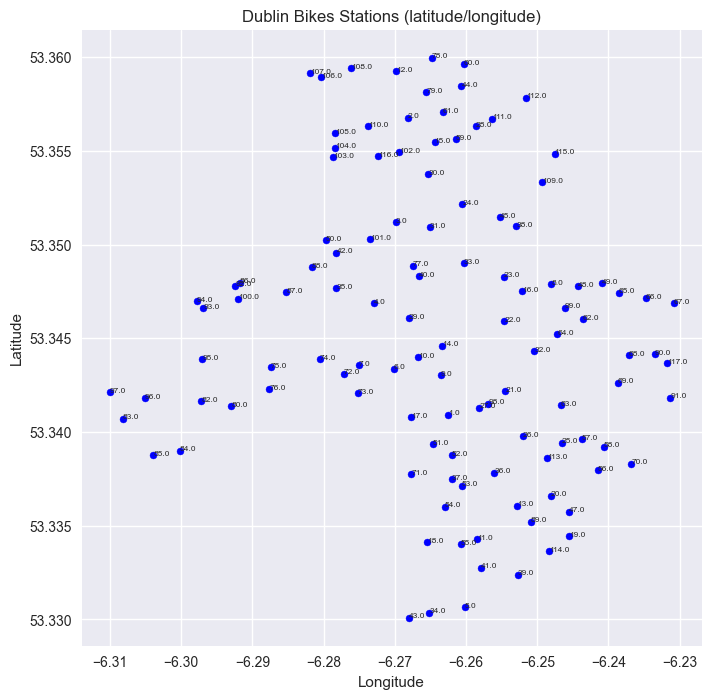
\includegraphics[width=0.80\linewidth]{figures/dublinbikes_station_map.png}
    \caption{Spatial distribution of DublinBikes stations used in this thesis (generated from the dataset station coordinates).}
    \label{fig:station_map}
\end{figure}

This thesis studies 30-minute prediction of \textit{available bikes} for all stations simultaneously. Stations are not independent from one another where demand can spill over to nearby stations, and many stations share commuting driven temporal patterns. Spatio- Temporal graph neural networks address this naturally by modeling stations as nodes on a graph and learning from both the spatial structure and temporal history \cite{yu2018stgcn,chen2021comparative}.  In addition to this, the work also integrates urban context using POI's from OpenStreetMaps, aggregated around stations using h3 hexagonal indexing \cite{osm_copyright,h3_docs}.


\section{Background}
Forecasting problems on networks are commonly addressed with models that combine graph learning ( to learn spatial dependencies) with temporal modeling ( to capture time varying dynamics). ST-GCN style approaches were initially popularized in traffic prediction and use graph convolutions for spatial structure together with temporal convolutions for efficient sequence learning \cite{yu2018stgcn}. Attention mechanisms improve on this idea By allowing the model to focus on the most relevant parts of recent history, which has been shown to improve spatio-temporal forecasting performances \cite{guo2019astgcn}.  In bike sharing attention based variants related graph based models have been evaluated directly on DublinBikes data, including attention based variants and different adjacency definitions \cite{chen2021comparative}.


\section{Motivation}
This work is mainly motivated by two practical needs. Firstly, short term predictions are only useful if they are at least reasonably accurate across the city and not just on average. If certain stations are consistently performing with larger errors the users near those stations receive lower quality information which can lead to be interpreted as bias in user experience \cite{yan2020fairness,zheng2021equality}. Second, predictions are more trustworthy when there is a clear explanation of what drives them. For that reason this thesis includes post-hoc explainability using Integrated gradients \cite{sundararajan2017ig} (via Captum \cite{captum_website}) and a mask-based edge explanation inspired by PGExplainer so as to identify which spatial connections are influencing the most for a target station prediction \cite{luo2020pgexplainer}.


\section{Problem Statement}
The technical problems is the learning to map from a multi station historical observations to multi station forecasts while respecting spatial structure across DublinBikes network. When given recent historical observations for all the stations, the goal is to predict the number of available bikes at each station for the next 30 minutes. 

To improve the prediction context beyond the raw station history, the thesis also considers static urban characteristics by integrating Points of Interest (POIs) derived from OpenStreetMap. POIs are aggregated around stations using H3 hexagonal indexing and used as station-level features \cite{osm_copyright,h3_docs}.


\section{Scope and Delimitations}
This thesis focuses on predicting \textit{available bikes} at DublinBikes stations using historical station status data from May 2024 to August 2025 \cite{smartdublin_dublinbikes_api}. Forecasts target a 30-minute prediction using 3 hours of historical context. The station graph is defined using geographic proximity between stations. Static urban context is incorporated using Points of Interest derived from OpenStreetMap and aggregated around stations using H3 hexagonal indexing \cite{osm_copyright,h3_docs}. This work does not optimize re balancing policies, simulate user routing behavior, or deploy a live production system. External signals such as weather, events, and pricing are also not included in the final models.

\section{Relevance to Human-Centred AI}
The human centered aspect is that outputs usefulness depend on not only total accuracy but also how reliable the system performs across different station as this can influence real world decisions. Two issues are the main aspect the first being transparency and other being bias aware evaluation \cite{yan2020fairness,zheng2021equality,eu_ai_act}. This thesis addresses both by combining station level performance analysis with explainability methods. In addition to feature attributions (Integrated Gradients), a PGExplainer-style edge mask is used to highlight influential spatial connections for selected predictions \cite{luo2020pgexplainer}.


\section{Research Questions and Objectives}
The research is guided by the following questions:
\begin{itemize}
    \item \textbf{RQ1:} How well can spatio-temporal graph neural networks predict short-term bike availability across all Dublin Bikes stations and would adding attention mechanism lead to increase in prediction ability?
    \item \textbf{RQ2:} Does incorporating contextual urban features (POIs) improve prediction quality beyond using availability history alone?
    \item \textbf{RQ3:} Can explainability methods provide useful insight into which time steps, stations, and POI features drive predictions?
\end{itemize}

To answer these questions, the objectives are:
\begin{itemize}
    \item Collect and clean Dublin Bikes historical availability data and align it into fixed time intervals.
    \item Construct a station graph based on spatial relationships.
    \item Implement and evaluate a baseline approach and graph-based deep learning models (ST-GCN, AST-GCN).
    \item Integrate POI-based static node features and measure the impact on performance.
    \item Apply explainability methods to interpret model decisions at temporal, spatial, and feature levels.
\end{itemize}

\section{Structure of the Thesis}
Chapter 2 reviews prior work on spatio-temporal forecasting, graph neural networks, bike-sharing prediction, and fairness/interpretability in mobility modeling. Chapter 3 describes the dataset, preprocessing, graph construction, and POI feature extraction. Chapter 4 details the modeling approach, training setup, and evaluation protocol. Chapter 5 presents quantitative results, station-level bias analysis, and explainability findings. Finally, Chapter 6 summaries the contributions, limitations, and future work directions.

\chapter{Literature Review}
\section{Spatio-temporal forecasting for networked mobility}
Bike sharing availability prediction is a spatio temporal forecasting problem where station behavior depends on both time ( like rush hours) and space( nearby stations acting as substitutes). Common time series and regression models can capture local trends but usually treat stations as independent which limits their ability to model inter station dependencies at the city scale. As a result recent researches are increasingly using deep learning models that combine temporal modeling with graph based representations of station networks.

\section{Graph neural networks for forecasting}
So much of the methodological foundation comes from traffic forecasting, where sensors form a graph and combines it with sequence to sequence recurrent modeling for time \cite{li2018dcrnn}. While it is effective recurrent models are often slow to train and less parallelizable.

ST-GCN introduced a fully convolutional approach that combines graph convolutions for spatial structure with temporal convolutions for time-series learning \cite{yu2018stgcn}.  Attention-based approaches provide another mechanism to capture complex dependencies. Graph WaveNet addresses this by learning an adaptive adjacency matrix in addition to using a given graph, enabling the model to discover latent node dependencies \cite{wu2019graphwavenet}. Attention-based approaches provide another mechanism to capture complex dependencies. GMAN uses multi-attention to model spatial and temporal interactions more flexibly, particularly for longer-horizon prediction \cite{zheng2020gman}.


\section{Bike Availability Prediction (Chen et al., 2021)}
This thesis is most directly inspired by Chen et al., who proposed an \textit{Attention-based Spatio-Temporal Graph Convolutional Network (AST-GCN)} for predicting the number of available bikes in bike-sharing schemes. Their work is particularly relevant because:
\begin{itemize}
    \item They evaluate on real bike-sharing datasets including \textbf{DublinBikes}.
    \item They extend a standard ST-GCN by adding an \textbf{attention mechanism} to improve performance.
    \item They discuss how different choices of \textbf{adjacency matrix construction} affect forecasting quality.
\end{itemize}

A practical takeaway from Chen et al. is that the adjacency design matters. A graph built only from physical distance can work well, but alternative adjacency definitions (e.g., correlation-based or demand-flow-based) may capture other different station relationships. Another key takeaway is that attention can help the model emphasize the most useful temporal context rather than treating all past observations equally.

\section{Gap Addressed by This Thesis}
While Chen et al. demonstrated a strong performance of AST-GCN, there is still some space to explore:
\begin{itemize}
    \item whether adding any \textbf{urban context} (e.g., POIs / land-use signals) improves prediction further,
    \item how attention affects different stations like some may benefit more than others,
    \item and how explainability can be used to make model behavior more transparent.
\end{itemize}

\section{Second comparison study: heterogeneity and context-aware modeling}
To complement Chen et al.\ with a secondary viewpoint, Zhao et al.\ propose a Robust Spatio-Temporal (RST) model with a dynamic hierarchical structure to better handle spatial and temporal heterogeneity in bike sharing prediction \cite{zhao2025rst}. Their motivation is that a single uniform model can under perform on irregular or non typical stations, and that incorporating multi-source context (such as POIs) helps explain station differences \cite{zhao2025rst}. Although their target is \emph{demand} rather than \emph{availability}, the core implication is directly relevant that is contextual features and heterogeneity aware modeling can reduce persistent, station-specific errors.

\section{Human-centered concerns: bias-aware evaluation and explainability}
Mobility prediction systems can fail unevenly across regions, which raises concerns about the fairness and who from the accurate predictions. Yan and Howe argue for fairness-aware evaluation in demand prediction for new mobility \cite{yan2020fairness}. Related work on equality of opportunity highlights that the model performance disparities can create unequal outcomes across contexts \cite{zheng2021equality}. In this thesis, a practical similarity is the station-level reliability that if some stations consistently have higher prediction error, users in those areas receive systematically worse information.

\section{Summary and positioning of this thesis}
Chen et al.\ provide a strong baseline for availability prediction and show the impact of attention and adjacency design, but the emphasis is mainly focused on accuracy comparisons \cite{chen2021comparative}. This thesis is extending on that work in mainly three ways. Firstly, it integrates interpretable POI-based urban context features (derived from OSM and aggregated using H3) to improve station representations, which also aligns with the evidence context improves bike sharing predictability. Second, it performs station level evaluation to identify any uneven reliability across the network as a bias-relevant quality issue \cite{yan2020fairness,zheng2021equality}. Third, it adds explainability at both feature level (Integrated Gradients) and graph-structure level (PGExplainer-style edge masks), supporting transparency beyond the aggregated metrics \cite{sundararajan2017ig,luo2020pgexplainer}. Overall, the literature motivates modeling bike availability as a spatio-temporal graph problem while also evaluating the reliability and interpretability aspects as human-centred requirements.

\chapter{Data Collection and Preparation}

\section{Data Sources}
\subsection{Dublin Bikes Availability Data}
The two main data sourced used in this thesis are Historical DublinBikes status data and OpenStreetMap (OSM) for POIs to add static urban context.


\subsubsection{DublinBikes station data.} The main datset is obtained from thesmart Sublin DublinBikes API portal \cite{smartdublin_dublinbikes_api}. The portal provides both static station metadata ( like location and station capacity) and dynamic status (like available bikes and free stands available)\cite{smartdublin_dublinbikes_api_resource}. To support long range modeling historical data from were collected and stored as monthly CSV files from May 2034 to August 2025. The raw combined dataset contains over nine million records where each is being represented with a view of a station's state at a given timestamp (station identifier, timestamp, and availability-related fields). The API documentation also mentions that the feed aligns with the General Bikeshare Feed Specification (GBFS), which supports consistent station-level access patterns \cite{smartdublin_dublinbikes_api}.


\subsubsection{OSM POI data.} POI information is extracted from OSM to represent station neighborhood context (e.g., education, retail, tourism).  Instead of downloading the global OSM planet file, The Ireland and northern Ireland regional part is extracted from Geofabric \cite{geofabrik_ireland}. This choice is practical for two reasons mainly being the file size is far smaller than global alternatives, making it manageable for local processing and reproducible experimentation \cite{geofabrik_ireland}. and its constantly being updated. POIs are parsed from the downloaded \texttt{.osm.pbf} extract using Pyrosm which is a library designed to read OSM PBF files into GeoDataFrames and extract POIs and other layers with standard filters \cite{pyrosm_docs}. 


Because OSM data is being used, attribution requirements are followed by crediting OpenStreetMap contributors and referencing the ODbL license guidance \cite{osm_copyright,osm_attribution}.

\section{Data Description}

After concatenating monthly DublinBikes CSV files, the raw dataset contains approximately 9.24 million rows with 16 columns (as printed in the notebook). Each observation corresponds to a station snapshot at a timestamp. The analysis focuses on the \textbf{available bikes} variable as the prediction target because it directly reflects whether a user can successfully pick up a bike at a station and retains station identifiers and timestamps for ensuring correct alignment across stations and consistent time indexing and window generation. 

\begin{table}[!h]
\centering
\caption{Dataset summary and preprocessing outcomes.}
\label{tab:data_summary}
\renewcommand{\arraystretch}{1.15}
\begin{tabular}{p{0.48\linewidth} p{0.42\linewidth}}
\hline
\textbf{Item} & \textbf{Value} \\
\hline
Selected data period (files) & 2024-05-01 to 2025-08-31 (16 monthly CSV files) \\
Raw combined dataset shape & 9,244,433 rows $\times$ 16 columns \\
Resampling frequency & 10 minutes (per-station) \\
Post-resampling dataset shape & 8,019,626 rows $\times$ 7 columns \\
Stations extracted & 115 stations \\
Wide matrix shape (time $\times$ stations) & 70,014 timestamps $\times$ 115 stations \\
Target range (available bikes) & min = 0, max = 40 \\
Missing values after fill & None (NaNs remaining: False) \\
\hline
\end{tabular}
\end{table}


The DublinBikes network used in this thesis contains \textbf{115 stations}. Station coordinates (latitude/longitude) are used both for visualization and for building spatial relationships between stations . After cleaning and resampling, the final station-by-time matrix contains \textbf{70,014} time steps at \textbf{10-minute} resolution across \textbf{115} stations, i.e., a shape of $(70014, 115)$ in wide format (time $\times$ stations). This wide representation is convenient for creating consistent spatio-temporal input tensors and ensures each training sample is containing a synchronized information across the full network.

\begin{figure}[h]
    \centering
    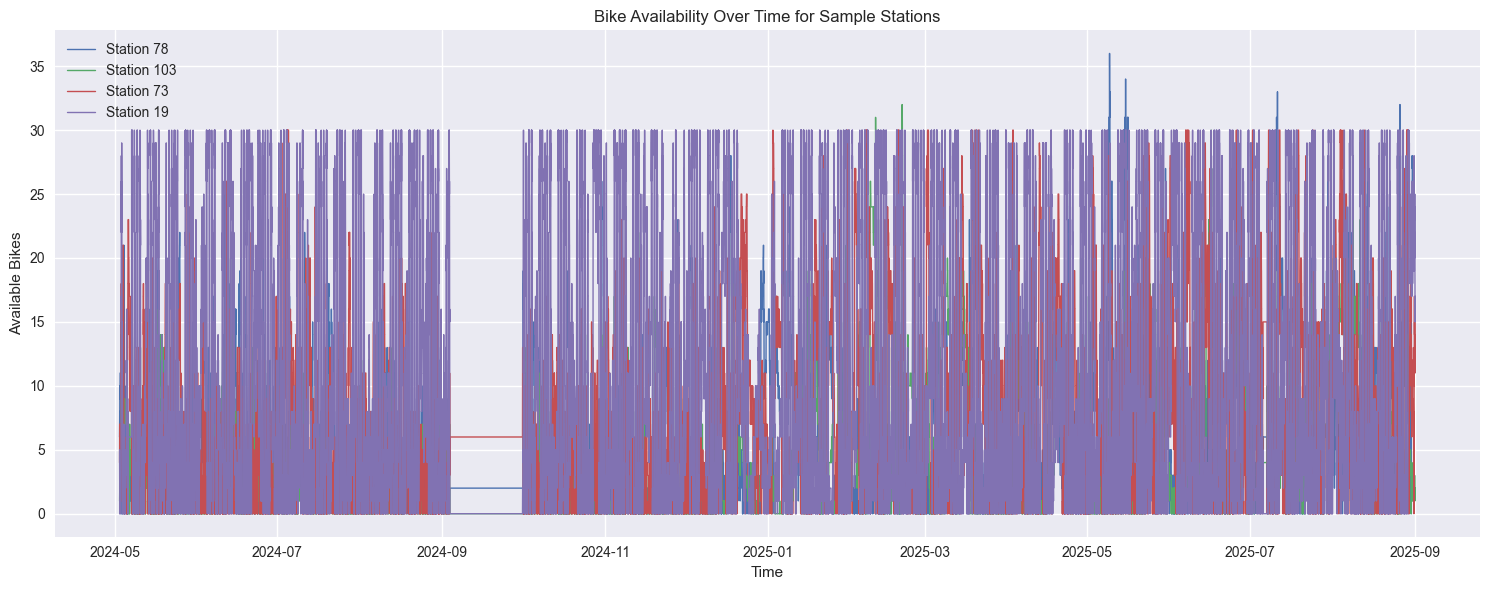
\includegraphics[width=0.95\linewidth]{figures/sample_station_timeseries.png}
    \caption{Bike availability over time for a small set of stations, illustrating strong temporal variation and short-term fluctuations.}
    \label{fig:data_sample_timeseries}
\end{figure}

\subsection{POI features.} POIs are treated as a static station-level attributes that describe the surrounding urban environment. The Geofabrik OSM extract is then filtered to POI-related tags (e.g., amenity/shop/tourism/leisure) and then mapped into six interpretable categories used in the notebook: \texttt{education}, \texttt{food\_drink}, \texttt{healthcare}, \texttt{shopping}, \texttt{tourism}, and \texttt{other}. Each station receives a POI-count vector summarizing nearby places, which helps distinguish stations that may have similar historical availability patterns but operate in different urban contexts (e.g., commuter hubs versus tourist-heavy locations).

\section{Data Insights and Visualization}

This subsection describes the key preprocessing decisions, exploratory insights, and data quality checks, including potential sources of bias in data representation.

\subsection{Temporal alignment and resampling.} DublinBikes status updates do not always arrive at the perfectly regular intervals, and individual stations can temporarily drop observations. To make the learning problem consistent, each station time series is resampled to a fixed \textbf{10-minute} frequency. Timestamps are parsed and converted to the local timezone (Europe/Dublin), then each station series is resampled and missing timestamps are filled using \textbf{forward-fill} followed by \textbf{back-fill}. This assumes that for the short gaps, the last observed state is a reasonable approximation until a new update arrives. After resampling, station series are pivoted to wide format (time $\times$ station) to support efficient multi-station modeling.

\subsection{Missingness and representation bias.} A station level missingness check is performed before resampling. Differences in missing data rates can lead to an uneven data quality across the network. For example, if some stations have frequent gaps, they may effectively contribute to a less reliable training signal, which can later be translated into higher prediction error for those particular stations. This motivates tracking station level data quality during preprocessing and later reporting station level performance, which is treated as a practical bias relevant indicator (unequal reliability across stations).

\begin{figure}[h]
    \centering
    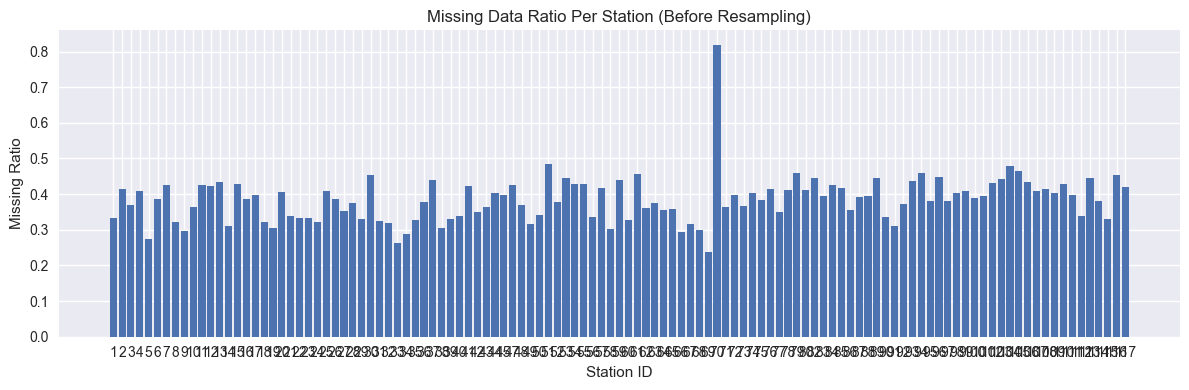
\includegraphics[width=0.95\linewidth]{figures/missing_ratio_per_station.png}
    \caption{Missing data ratio per station before resampling. Stations with higher missingness may provide lower-quality learning signal, which can later contribute to uneven prediction reliability.}
    \label{fig:data_missing_ratio}
\end{figure}

\subsection{Exploratory patterns.} Several plots in the notebook highlight regular usage structure:
(1) availability time series for selected stations shows strong short-term variability and repeated cycles;
(2) average daily patterns show time-of-day structure consistent with commuting and daily routines and
(3) weekly averages reveal differences between weekday and weekend usage. These patterns justify the use of cyclical calendar features and spatio-temporal modeling rather than treating the process as stationary noise.

\begin{figure}[h]
    \centering
    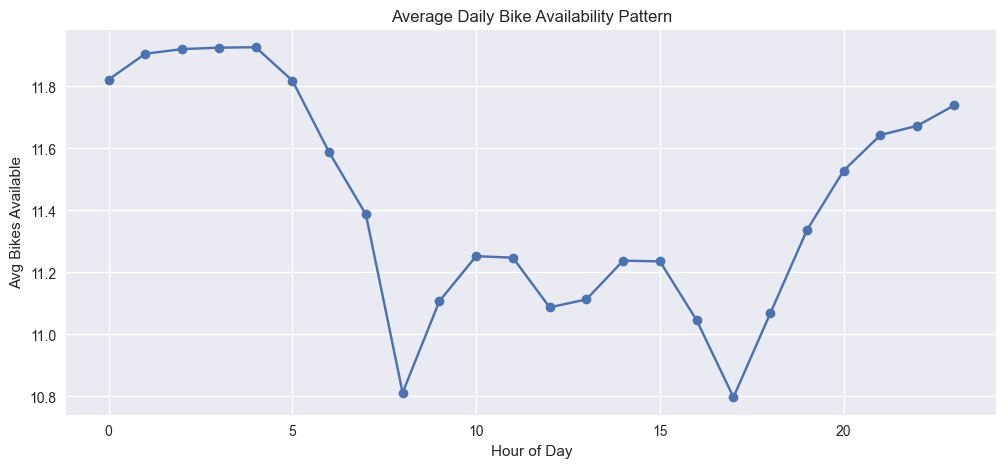
\includegraphics[width=0.90\linewidth]{figures/avg_daily_pattern.png}
    \caption{Average daily bike availability pattern across the network, showing clear time-of-day structure.}
    \label{fig:data_avg_daily}
\end{figure}

\begin{figure}[h]
    \centering
    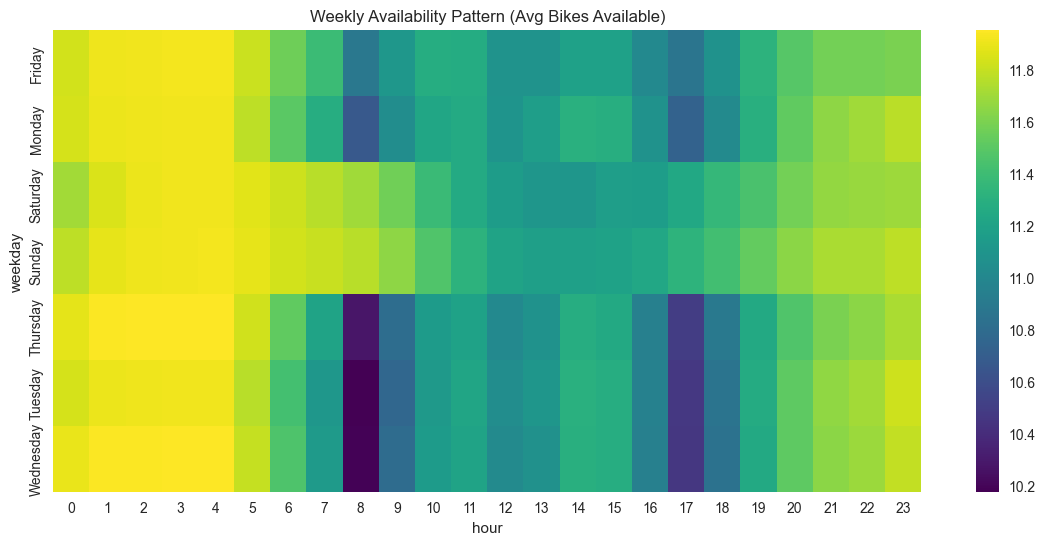
\includegraphics[width=0.90\linewidth]{figures/weekly_pattern.png}
    \caption{Weekly availability pattern (average bikes available), highlighting differences between weekdays and weekends.}
    \label{fig:data_weekly}
\end{figure}

\subsection{Feature construction for modeling.} The final supervised learning dataset is created using a sliding-window formulation. Inputs use \textbf{3 hours of history} (18 timesteps at 10-minute resolution) and targets use a \textbf{30-minute horizon} (3 timesteps). The notebook constructs a tensor $X$ with shape $(69994, 18, 115, 5)$ and $Y$ with shape $(69994, 3, 115)$. 
The feature dimension includes the standardized availability signal plus cyclical encodings for hour-of-day and day-of-week (sine and cosine pairs). Standardization is applied to stabilize optimization, while evaluation is reported in the original bike-count scale for interpretability.

\begin{table}[!htbp]
\centering
\small
\caption{Supervised learning setup and train/validation/test split.}
\label{tab:window_split}
\renewcommand{\arraystretch}{1.15}
\begin{tabular}{>{\raggedright\arraybackslash}p{0.34\linewidth} >{\raggedright\arraybackslash}p{0.58\linewidth}}
\hline
\textbf{Item} & \textbf{Value} \\
\hline
Sampling interval & 10 minutes \\
History length ($T_{in}$) & 18 timesteps (3 hours) \\
Forecast horizon ($T_{out}$) & 3 timesteps (30 minutes) \\
Input tensor $X$ shape & (69,994, 18, 115, 5) \\
Target tensor $Y$ shape & (69,994, 3, 115) \\
Train split & 48,995 samples; $X$: (48,995, 18, 115, 5), $Y$: (48,995, 3, 115) \\
Validation split & 10,499 samples; $X$: (10,499, 18, 115, 5), $Y$: (10,499, 3, 115) \\
Test split & 10,500 samples; $X$: (10,500, 18, 115, 5), $Y$: (10,500, 3, 115) \\
\hline
\end{tabular}
\end{table}

\FloatBarrier



\subsection{POI aggregation using H3.} To connect POIs to stations, station coordinates and POI geometries are mapped into H3 hexagonal cells and aggregated at a fixed resolution. The H3-based join provides a consistent spatial neighborhood definition and avoids the complexity of any repeated point-in-polygon operations. The result is a POI feature matrix of shape $(115, 6)$ (stations $\times$ POI categories), which is then standardized before being fused into the POI-augmented model variants.


\begin{table}[H]
\centering
\small
\caption{Input feature dimensions for base and POI-augmented variants.}
\label{tab:feature_schema}
\renewcommand{\arraystretch}{1.15}
\begin{tabular}{>{\raggedright\arraybackslash}p{0.50\linewidth} >{\raggedright\arraybackslash}p{0.42\linewidth}}
\hline
\textbf{Input representation} & \textbf{Shape / dimension} \\
\hline
Base (no POI) feature dimension & $F=5$ \\
POI feature matrix & (115, 6) \\
POI-augmented feature dimension & $F=11$ (5 temporal + 6 POI) \\
Example (train) base tensor & $X_{train}$: (48,995, 18, 115, 5) \\
Example (train) POI-augmented tensor & $X_{train}^{POI}$: (48,995, 18, 115, 11) \\
\hline
\end{tabular}
\end{table}



\begin{figure}[h]
    \centering
    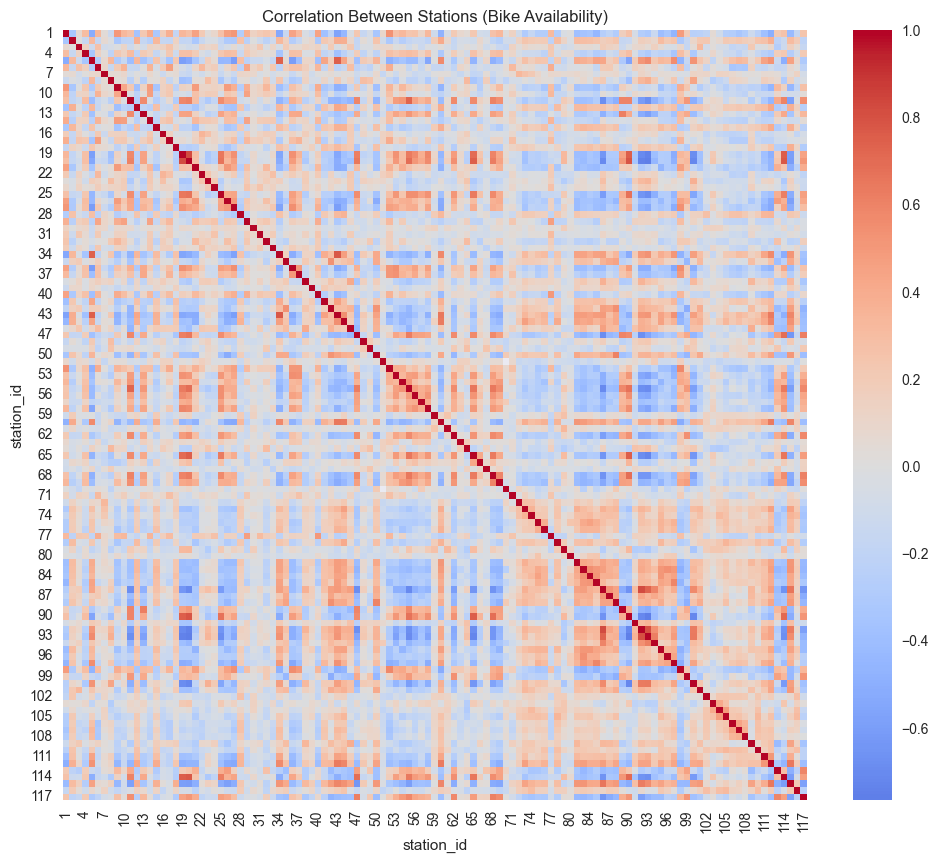
\includegraphics[width=0.95\linewidth]{figures/station_correlation.png}
    \caption{Correlation between stations based on bike availability time series. This provides evidence that stations are interdependent rather than independent signals.}
    \label{fig:data_station_corr}
\end{figure}

\chapter{AI Modeling}

In this chapter we go through the model development process used to predict DublinBikes availability using spatio temporal graph neural networks. The main goal is to learn a function that maps a short history of networks wide station states to a multi step forecast while also respecting i) temporal structure (daily/weekly patterns) and (ii) spatial dependence between nearby stations. . Model development was implemented in PyTorch and evaluated using a test set which was held out, with checkpoints selected based on validation MAE. Throughout the modeling process, emphasis was placed on controlled comparisons like only one design component (attention or POI features) is changed at a time so that improvements can be attributed to specific modeling choices rather than unrelated implementation differences. The modeling approach follows prior ST-GCN-based availability prediction studies and adapts them to the DublinBikes setting \cite{chen2021comparative,yu2018stgcn}.


\begin{figure}[!htbp]
    \centering
    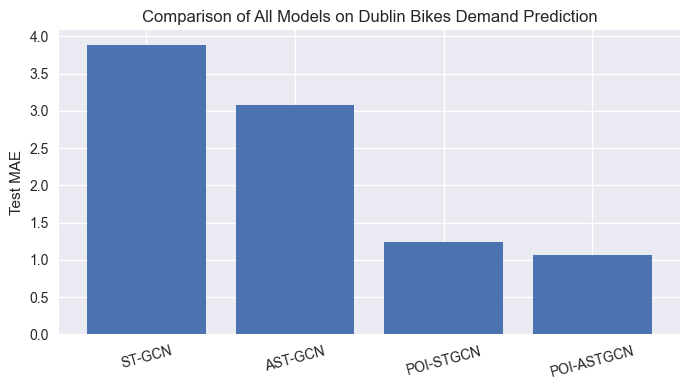
\includegraphics[width=0.95\linewidth]{figures/model_comparison_all.png}
    \caption{Comparison of all models on Dublin Bikes demand prediction (notebook title: ``Comparison of All Models on Dublin Bikes Demand Prediction'').}
    \label{fig:model_comparison_all}
\end{figure}

\section{Model Selection and Development}
\subsection{Forecasting formulation}
The supervised learning setup is following the sliding-window formulation discussed in data. Each training sample uses a history length of $T_{in}=18$ timesteps (3 hours at 10-minute resolution) across $N=115$ stations to predict the next $T_{out}=3$ timesteps (30 minutes). Inputs are represented as
$X \in \mathbb{R}^{B \times T_{in} \times N \times F}$ and targets as
$Y \in \mathbb{R}^{B \times T_{out} \times N}$, where $B$ is the batch size and $F$ is the feature dimension. In the base setting, $F=5$ includes the standardized availability signal and cyclical time encodings (hour-of-day and day-of-week sine/cosine pairs). This formulation is well-suited to short-horizon operational prediction because it focuses the model on recent dynamics while still capturing recurring temporal structure through the calendar encodings.

\textbf{Model formulation.} Let $x_{t} \in \mathbb{R}^{N \times F}$ denote the station-feature matrix at time index $t$. For each training sample, the input is a sequence of the most recent $T_{in}$ matrices and the target is the next $T_{out}$ availability vectors:
\[
X_t = [x_{t-T_{in}+1}, \ldots, x_t] \in \mathbb{R}^{T_{in} \times N \times F}, \quad
Y_t = [y_{t+1}, \ldots, y_{t+T_{out}}] \in \mathbb{R}^{T_{out} \times N},
\]
where $y_t \in \mathbb{R}^{N}$ is the available-bikes value for all stations at time $t$. The learning objective is to fit a function $f_{\theta}$ such that $\hat{Y}_t = f_{\theta}(X_t, \tilde{A})$ minimizes prediction error over the training set, where $\tilde{A}$ is the normalized adjacency matrix and $\theta$ are model parameters.

\subsection{Graph construction and normalization}
Spatial structure is encoded using a station graph which is built from geographic proximity. A binary adjacency matrix $A \in \{0,1\}^{N \times N}$ is constructed using the Haversine distance between station coordinates with a 500m threshold, and self-connections are included to preserve each node’s own signal. The 500m threshold was selected as a reasonable walking distance that can represent realistic substitution behavior (like when users are walking to a nearby station when their preferred station is empty or full), while keeping the graph sparse enough to avoid any over-smoothing.

Before graph convolution, the adjacency is symmetrically normalized as
$\tilde{A} = D^{-\frac12}(A + I)D^{-\frac12}$, which stabilizes message passing and is commonly used in graph convolutional networks \cite{kipf2017gcn}. This normalized adjacency $\tilde{A}$ is used consistently across all the graph-based models for comparability.

\subsection{Baseline models}
A naive persistence baseline is used as a minimum reference point which can be defined by the last observed availability value is repeated for all future steps in the horizon. This baseline is simple but meaningful in a short-horizon forecasting, because many stations change gradually over 10--30 minutes and the baseline often performs better than what we expect. Improvements over this baseline can provide evidence that the model is actually learning actionable structure rather than simply smoothing  of the input.

\subsection{ST-GCN architecture}
The first deep model is a Spatio-Temporal Graph Convolutional Network (ST-GCN), implemented as stacked spatio-temporal convolution blocks. The model alternates between:
(i) spatial graph convolution using $\tilde{A}$ to mix information across neighboring stations, and
(ii) temporal convolution across the input history to capture short-term dynamics.
In the notebook implementation, two ST-convolution blocks are followed by a temporal convolution layer and a linear projection being applied per station to output $T_{out}$ future values. This design is computationally efficient because temporal convolutions are parallelizable and avoid recurrent unrolling. In practice, this makes the model easier to train on large datasets and less sensitive to exploding/vanishing gradients compared to the deep recurrent baselines.

\subsection{AST-GCN: adding temporal attention}
To better capture which timesteps in the input history are the most relevant for the forecast, an attention-based extension is being used. The AST-GCN model keeps the same graph-convolution backbone but inserts a Temporal Attention Module (TAM) that applies multi-head self-attention over the time dimension (per node) using PyTorch’s \texttt{MultiheadAttention} \cite{pytorch_mha}. Conceptually, attention allows the model to reweigh the historical timesteps dynamically instead of relying only on fixed-size temporal kernels, building on the general self-attention mechanism introduced in Transformer models \cite{vaswani2017attention}. This is helpful when recent timesteps are not equally informative (which for example, sudden availability drops or spikes), because the model can focus on the most predictive parts of the window. In the notebook, attention uses 4 heads and a small dropout value to reduce overfitting.

\subsection{POI-augmented variants}
A limitation of purely historical availability features is that stations with similar short-term patterns may still differ due to the surrounding land use context (e.g., being commuter vs.\ tourist areas). To address this, static POI features derived from OpenStreetMap and aggregated using h3 \cite{osm_copyright,geofabrik_ireland,h3_docs}.
 are concatenated to the per-station feature vectors. In implementation terms, a station-level POI matrix of shape $(N,6)$ is broadcast across batch and time and concatenated to $X$ along the feature axis, producing $F=11$ for POI models. Two additional variants are trained:
\textbf{POI-STGCN} and \textbf{POI-ASTGCN}. This allows the contribution of POIs and attention to be isolated through controlled comparisons. Importantly, POIs are static here, so the model learns how context modulates dynamics (e.g., similar temporal patterns may shift in magnitude or volatility depending on neighborhood characteristics).

\begin{table}[H]
\centering
\small
\caption{Model variants and core configuration used in the notebook implementation.}
\label{tab:model_configs}
\renewcommand{\arraystretch}{1.15}
\begin{tabular}{>{\raggedright\arraybackslash}p{0.30\linewidth} >{\raggedright\arraybackslash}p{0.62\linewidth}}
\hline
\textbf{Component} & \textbf{Setting} \\
\hline
Graph construction & Haversine distance threshold = 500m; $N=115$ stations; self-loops included \\
Adjacency normalisation & $\tilde{A} = D^{-\frac12}(A+I)D^{-\frac12}$ \cite{kipf2017gcn} \\
Input / output lengths & $T_{in}=18$ (3 hours), $T_{out}=3$ (30 minutes) \\
Base feature dimension & $F=5$ (availability\_z + hour\_sin/cos + dow\_sin/cos) \\
POI feature dimension & 6 POI categories; POI models use $F=11$ \\
ST-GCN channels & spatial\_channels = 16, out\_channels = 32, kernel\_size = 3 \\
AST-GCN attention & num\_heads = 4; temporal self-attention per node \cite{vaswani2017attention,pytorch_mha} \\
Optimisation & Adam, lr $=10^{-3}$, weight decay $=10^{-5}$ \cite{kingma2015adam} \\
Batch size & 64 \\
Checkpoint selection & Best validation MAE saved and reloaded for testing \\
\hline
\end{tabular}
\end{table}

\section{Hyper Parameter Tuning}
Hyperparameter tuning was performed using the validation set MAE as the selection criterion. Given the relatively large training set and the goal of maintaining reproducibility, tuning focused on a small number of high-impact parameters while keeping the training pipeline fixed across model variants. Rather than running an extensive automated search, the approach prioritized stable convergence and fair comparisons between variants.

\subsection{Parameters considered}
The main parameters that were explored are:
\begin{itemize}
    \item \textbf{Model capacity:} The number of channels in spatial/temporal layers (e.g., 16/32) to balance underfitting vs.\ overfitting.
    \item \textbf{Temporal receptive field:} kernel size in temporal convolutions (kernel\_size $=3$ in the final setup), controlling how local temporal patterns are aggregated.
    \item \textbf{Optimization:} learning rate and weight decay under Adam \cite{kingma2015adam}. The final configuration uses lr $=10^{-3}$ and weight decay $=10^{-5}$, which provided stable convergence without excessive regularization.
    \item \textbf{Attention configuration (AST-GCN):} number of heads (4 heads) and dropout, controlling attention flexibility and regularization \cite{vaswani2017attention}.
\end{itemize}
In addition, the same batch size and loss function were used across experiments to ensure that the observed differences reflect model design choices (graph convolution, attention, and POI fusion) rather than any training instability.

\subsection{Training protocol and check pointing}
All models are trained with mini batches (batch size 64) using MAE loss (implemented as \texttt{nn.L1Loss}). Each epoch is shown to report train and validation MAE, and the model state with the lowest validation MAE is saved as a checkpoint. This is a practical form of early stopping and avoids selecting models based on the test set. For comparability across variants, the same training loop and stopping rule are used for ST-GCN/AST-GCN and their POI-augmented counterparts. Where training curves differed, preference was given to settings that produced smooth validation improvement without oscillation, as these were more robust across repeated runs.

\section{Model Evaluation}
\subsection{Evaluation metrics}
Model performance is evaluated primarily using Mean Absolute Error (MAE) because it is directly interpretable in the scale of the target and it aligns with the optimization loss used during training. 

\textbf{Mean Absolute Error (MAE).} MAE measures the average absolute difference between predicted and true values. For predictions $\hat{y}$ and ground truth $y$ over stations $n \in \{1,\ldots,N\}$ and forecast steps $k \in \{1,\ldots,T_{out}\}$, MAE is:
\[
\mathrm{MAE} = \frac{1}{N \cdot T_{out}} \sum_{n=1}^{N}\sum_{k=1}^{T_{out}} \left| \hat{y}_{n,k} - y_{n,k} \right|.
\]
MAE is reported in \emph{bike units} (after reversing any normalization), which makes it easy to interpret operationally (e.g., an MAE of 3 means an average error of about 3 bikes per station per forecast step).So, the more close to 0 the MAE is the better the model accuracy.

MAE is computed over all stations and all forecast steps in the horizon. In addition to aggregate MAE, per-station MAE is also computed to identify any locations where prediction quality is systematically worse, which is useful for diagnosing uneven reliability across the network. Station-level analysis also supports human-centered evaluation because it highlights where users would experience less reliable predictions.

MAE is preferred here over squared-error metrics such as MSE/RMSE because it is directly interpretable in the original units (bikes) and is less dominated by occasional large errors at a small number of stations or time periods, which makes comparisons between model variants easier to communicate in an operational setting.

\subsection{Comparison framework}
Evaluation is structured around controlled comparisons:
(i) naive persistence baseline vs.\ learned models (value of learning),
(ii) ST-GCN vs.\ AST-GCN (value of attention),
(iii) base models vs.\ POI-augmented models (value of contextual features), and
(iv) POI-STGCN vs.\ POI-ASTGCN (interaction of attention and context).
This comparison strategy ensures that improvements can be attributed to specific design choices rather than incidental implementation differences. Results are reported at both network level (overall MAE) and also at the station level to provide a clearer picture of how improvements are distributed across the city.

\begin{figure}[!htbp]
    \centering
    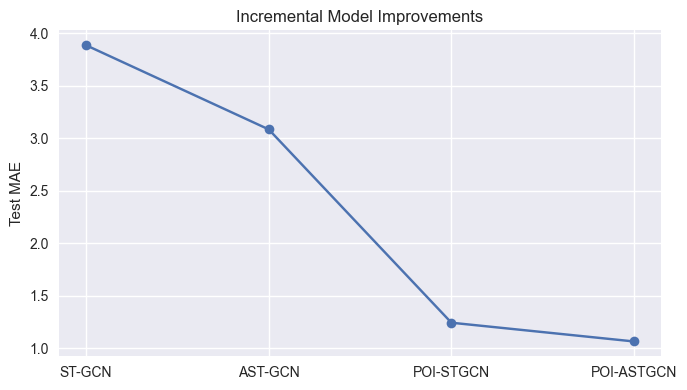
\includegraphics[width=0.95\linewidth]{figures/incremental_improvements.png}
    \caption{Incremental model improvements (notebook title: ``Incremental Model Improvements'').}
    \label{fig:incremental_improvements}
\end{figure}

\begin{figure}[!htbp]
    \centering
    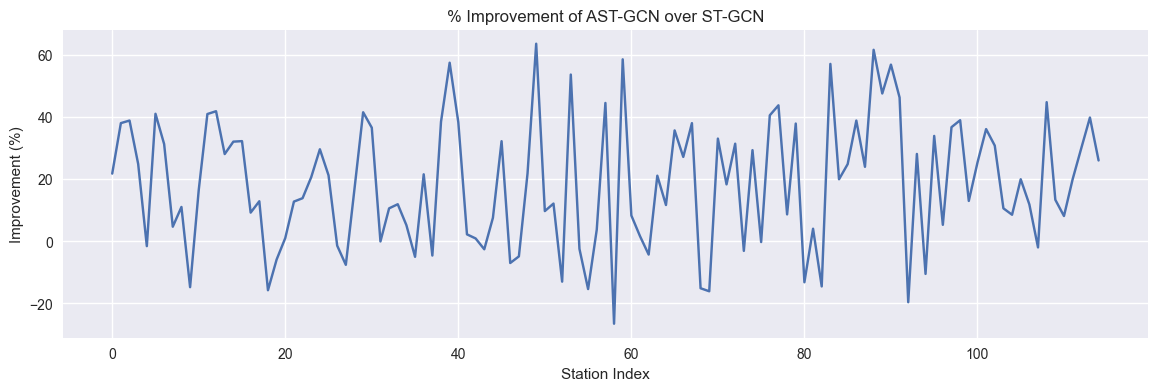
\includegraphics[width=0.95\linewidth]{figures/astgcn_improvement_pct.png}
    \caption{\% improvement of AST-GCN over ST-GCN at station level (notebook title: ``\% Improvement of AST-GCN over ST-GCN'').}
    \label{fig:astgcn_improvement_pct}
\end{figure}


\chapter{Results and Discussion}

\section{Results}
This section reports the predictive performance of the proposed spatio-temporal graph models on the test set which is held out and remains unseen to the model. Performance is measured using Mean Absolute Error (MAE) in \emph{bike units}, where lower values indicate better accuracy and the ideal score is 0 (perfect prediction). In practical terms, an MAE close to 1 means the model is off by roughly one bike on average (per station per forecast step).

\subsection{Overall predictive performance}
A simple persistence baseline (predicting the last observed value forward) performs poorly, highlighting that bike availability is not well approximated by a stationary or a purely local rule. The base ST-GCN substantially improves upon this baseline, confirming that modeling spatial dependency between stations and temporal dynamics together is effective for the DublinBikes setting.

Adding temporal attention (AST-GCN) further reduces error compared to ST-GCN, indicating that attention can help the model emphasize the most informative parts of the recent history when producing short-horizon forecasts. The largest improvement comes from incorporating static neighborhood context via POI features. Both POI-augmented variants (POI-STGCN and POI-ASTGCN) outperform their non-POI counterparts by a wide margin, with POI-ASTGCN achieving the best overall accuracy.

\begin{figure}[!htbp]
    \centering
    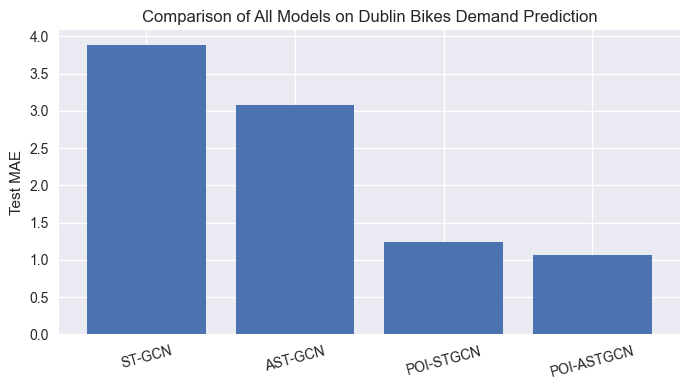
\includegraphics[width=0.92\linewidth]{figures/model_comparison_all.png}
    \caption{Overall test MAE comparison across baseline and model variants. Lower is better.}
    \label{fig:overall_model_comparison}
\end{figure}

\begin{table}[!htbp]
\centering
\caption{Test-set performance (MAE in bike units). Percent improvement is shown relative to the naive persistence baseline.}
\label{tab:overall_results}
\renewcommand{\arraystretch}{1.15}
\begin{tabular}{lccc}
\hline
\textbf{Model} & \textbf{Test MAE} & \textbf{Improvement vs Naive} \\
\hline
Naive (persistence) & 11.5031 & -- \\
ST-GCN & 3.8842 & 66.23\% \\
AST-GCN & 3.0828 & 73.20\% \\
POI-STGCN & 1.2425 & 89.20\% \\
POI-ASTGCN & 1.0639 & 90.75\% \\
\hline
\end{tabular}
\end{table}


\subsection{Station-level performance (bias-relevant differences)}
While the overall MAE is strong, errors are not evenly distributed across stations. Table~\ref{tab:station_extremes} highlights the best and worst station-level MAE values for ST-GCN and AST-GCN (as printed in the notebook). This station-to-station variability is important from a human-centered perspective that is if certain stations consistently have higher error, commuters depending on those locations may receive less reliable predictions, and operators may make poorer re balancing decisions for those areas which could lead to less available bikes than the demand.

\begin{figure}[!htbp]
    \centering
    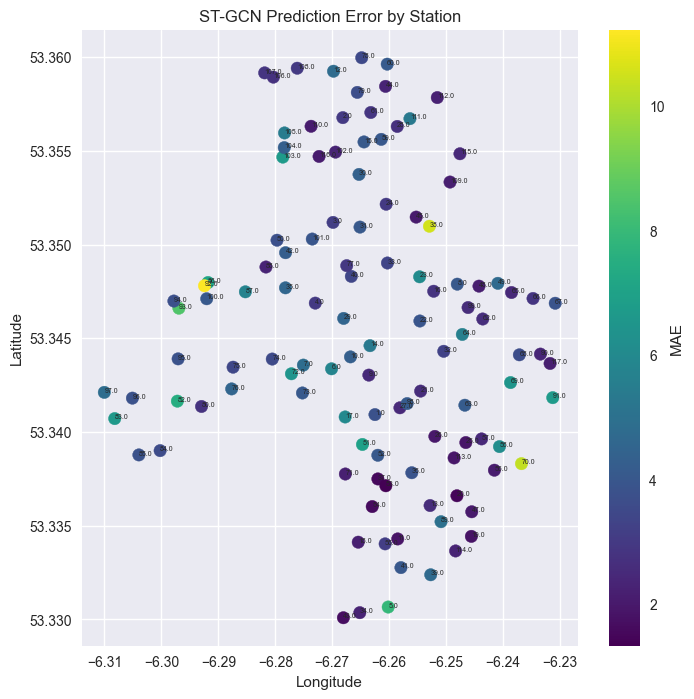
\includegraphics[width=0.92\linewidth]{figures/stgcn_error_by_station.png}
    \caption{ST-GCN station-level MAE visualized spatially.}
    \label{fig:stgcn_station_map}
\end{figure}

\begin{figure}[!htbp]
    \centering
    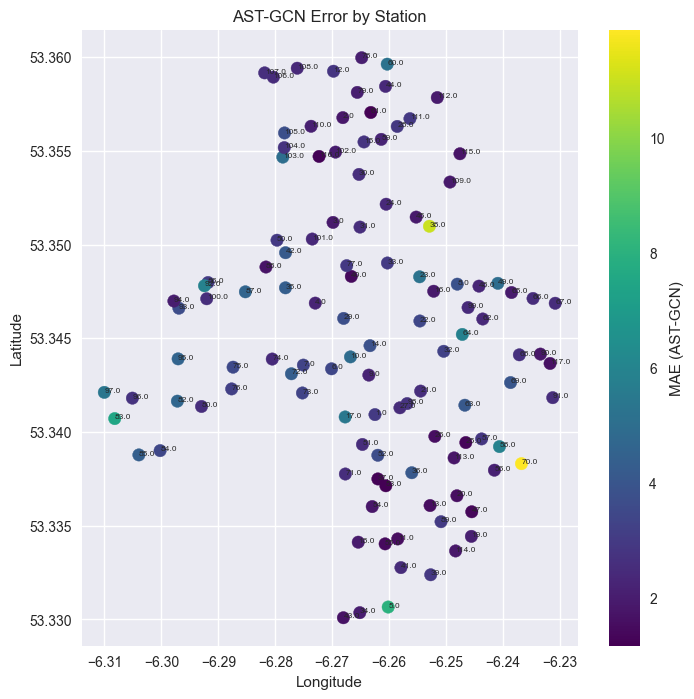
\includegraphics[width=0.92\linewidth]{figures/astgcn_error_by_station.png}
    \caption{AST-GCN station-level MAE visualized spatially.}
    \label{fig:astgcn_station_map}
\end{figure}

\begin{table}[!htbp]
\centering
\caption{Best and worst station MAE. Station identifiers here refer to the station index used in the model tensors.}
\label{tab:station_extremes}
\renewcommand{\arraystretch}{1.15}
\begin{tabular}{lccc}
\hline
\textbf{Model} & \textbf{Best station (index, MAE)} & \textbf{Worst station (index, MAE)} \\
\hline
ST-GCN & (51, 1.3264) & (89, 11.2262) \\
AST-GCN & (51, 1.1652) & (68, 11.8735) \\
\hline
\end{tabular}
\end{table}


\section{Discussion}
This section interprets the results in a relation to the research questions and objectives, discusses the unexpected behavior, and frames the findings through a human-centered lens (transparency, fairness, and practical impact).

\section{Recap of research questions and objectives}
The project set out to answer the following questions:

\begin{itemize}
    \item \textbf{RQ1:} How well can spatio-temporal graph neural networks predict short-term bike availability across all Dublin Bikes stations and would adding attention mechanism lead to increase in prediction ability?
    \item \textbf{RQ2:} Does incorporating contextual urban features (POIs) improve prediction quality beyond using availability history alone?
    \item \textbf{RQ3:} Can explainability methods provide useful insight into which time steps, stations, and POI features drive predictions?
\end{itemize}

\subsection{Summary and interpretation of findings}
\subsubsection{RQ1: Spatio-temporal GNN performance and the impact of attention}
The results support the claim that the spatio-temporal graph neural networks can predict short-term DublinBikes availability effectively across the full network. Compared to the naive persistence baseline, ST-GCN achieves a large reduction in MAE (Table~\ref{tab:overall_results}). This indicates that availability is not well explained by “no-change” behavior and that learning both temporal dynamics and spatial relationships between stations is very important. Practically, stations influence each other through nearby substitution (users walking to alternatives) and shared movement corridors. Graph-based modeling is well suited to this type of structured dependency, consistent with ST-GCN-style forecasting literature \cite{yu2018stgcn}.

Adding an attention mechanism further improves the prediction ability. AST-GCN improves on ST-GCN in overall MAE (Table~\ref{tab:overall_results}), suggesting that the model benefits from reweighting the input window rather than treating all 3 hours of history as equally informative. This aligns with attention-based spatio-temporal forecasting methods \cite{guo2019astgcn}. The station-level improvement plot (Figure~\ref{fig:ast_improvement_pct}) also shows that attention benefits are not uniform like some stations gain more than others. A realistic interpretation is that attention is most valuable where short-term dynamics depend on a few highly informative moments (e.g., rapid depletion or refilling) rather than smooth trends.

\begin{figure}[!htbp]
    \centering
    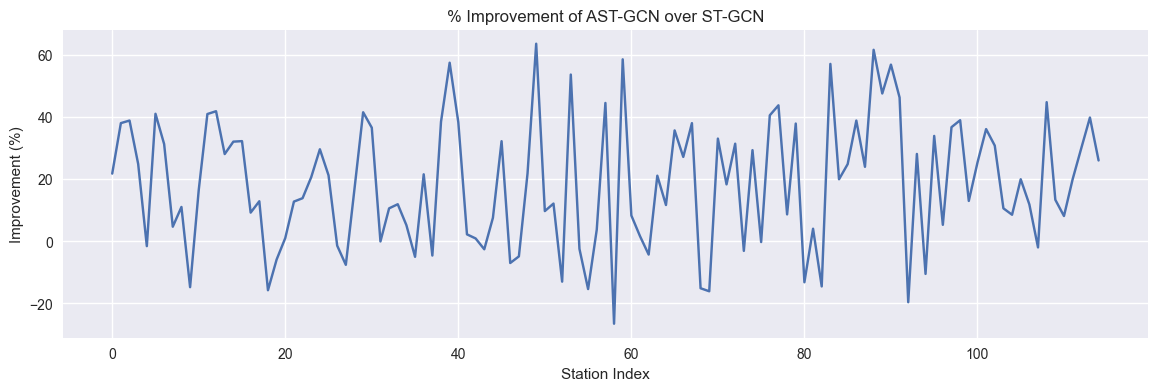
\includegraphics[width=0.92\linewidth]{figures/astgcn_improvement_pct.png}
    \caption{\% improvement of AST-GCN over ST-GCN at station level. Positive values indicate stations that benefit more from attention.}
    \label{fig:ast_improvement_pct}
\end{figure}

However, station-level extremes remain important. Even when the average improves, some stations can still be difficult to predict (Table~\ref{tab:station_extremes}). This matters because users experience the system locally: a strong average performance can still hide “weak stations” where forecasts are consistently less reliable. For real-world use, this suggests that evaluation should include not only a global MAE but also station-level distributions and outliers.

\subsubsection{RQ2: Does urban context (POIs) improve prediction beyond history alone?}
The strongest finding is that incorporating POI context substantially improves prediction quality beyond availability history alone. Both POI-augmented models outperform their history-only counterparts, with POI-ASTGCN producing the best MAE overall (Table~\ref{tab:overall_results}). This supports the hypothesis that station behavior is shaped not only by the recent availability but also by persistent local context. Two stations can look similar in the last hour, yet differ in the next 30 minutes due to differences in land use and activity (e.g., retail/nightlife/tourism versus commuter-oriented areas). POIs provide a structured proxy for these stable station “types”.

From an operational perspective, the size of the improvement is significant. Once MAE approaches roughly one bike per station per forecast step, the predictions are becoming far more actionable for both commuters (trip planning) and operators (anticipating shortages and re balancing). At the same time, POIs are static and cannot fully represent day-to-day shocks (events, weather, disruptions). The result should therefore be interpreted as context greatly improves baseline predictability, but it does not remove the need for dynamic signals if the goal is robustness under unusual conditions. This is consistent with broader work showing value from multi-source features while also noting that system heterogeneity and non-stationary remain challenges \cite{zhao2025rst}.

\subsubsection{RQ3: Explainability insights across time, space, and POI features}
Explainability methods provide useful insight into what drives predictions at multiple levels.
\begin{figure}[!htbp]
    \centering
    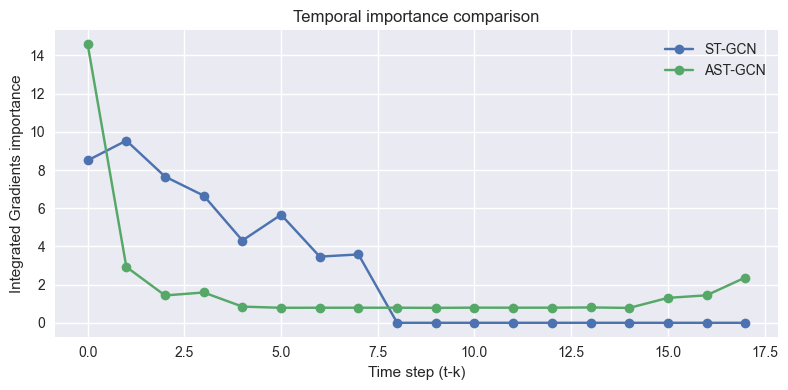
\includegraphics[width=0.92\linewidth]{figures/temporal_importance_comparison.png}
    \caption{Integrated Gradients temporal attribution for ST-GCN vs AST-GCN}
    \label{fig:ig_temporal}
\end{figure}

\textbf{Time-step importance.} Integrated Gradients (IG) indicates that more recent timesteps tend to dominate attribution for short-horizon forecasting (Figure~\ref{fig:ig_temporal}). This is a valuable sanity check: the model is relying on plausible evidence aligned with the prediction horizon rather than spurious long-range effects \cite{sundararajan2017ig,captum_website}. For stakeholders, this also gives a simple narrative: “the most recent station behavior matters most for the next 30 minutes”.

\begin{figure}[!htbp]
    \centering
    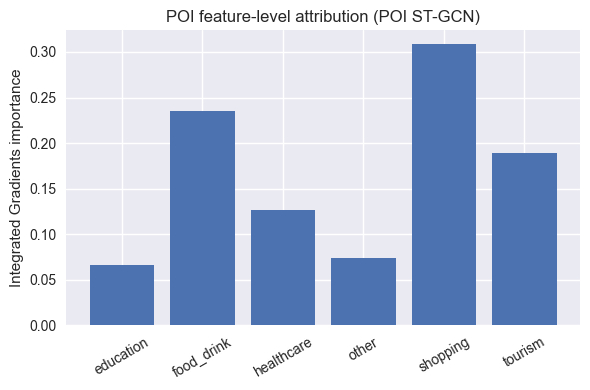
\includegraphics[width=0.75\linewidth]{figures/poi_feature_attribution.png}
    \caption{Integrated Gradients attribution over POI categories.}
    \label{fig:ig_poi_feat}
\end{figure}

\textbf{POI feature importance.} For POI-augmented models, IG over POI channels is not uniform (Figure~\ref{fig:ig_poi_feat}). Higher attribution for categories such as shopping, food\_drink, and tourism supports a plausible interpretation of how land use shapes station dynamics. These attributions do not prove causality, but they do show that POIs are being used in a structured way rather than ignored as noise, which improves transparency when communicating model behavior.

\textbf{Station-to-station influence.} The mask-based edge explanation (PGExplainer-style) provides ranked influential incoming edges for a target station (Table~\ref{tab:pgexplainer_edges}) \cite{luo2020pgexplainer}. The explanation is sparse: a small set of neighbors carries most of the weight. This is useful in practice because it produces human-readable statements such as “these nearby stations contributed most to the prediction”. It also supports debugging. For example, if the top edges repeatedly point to non-local or unintuitive stations, that can flag issues in graph construction or feature leakage.

\begin{table}[!htbp]
\centering
\caption{Top incoming edges for the target station (station\_id=1) from the notebook’s mask-based edge explanation (PGExplainer-style). Weights are in $[0,1]$ after the sigmoid mask.}
\label{tab:pgexplainer_edges}
\renewcommand{\arraystretch}{1.15}
\begin{tabular}{ccc}
\hline
\textbf{Rank} & \textbf{Edge (from $\rightarrow$ to)} & \textbf{Weight} \\
\hline
1  & 14 $\rightarrow$ 1 & 0.9064 \\
2  & 10 $\rightarrow$ 1 & 0.8984 \\
3  & 9  $\rightarrow$ 1 & 0.8965 \\
4  & 27 $\rightarrow$ 1 & 0.8838 \\
5  & 98 $\rightarrow$ 1 & 0.8799 \\
6  & 52 $\rightarrow$ 1 & 0.8479 \\
7  & 37 $\rightarrow$ 1 & 0.8016 \\
8  & 71 $\rightarrow$ 1 & 0.0948 \\
9  & 53 $\rightarrow$ 1 & 0.0937 \\
10 & 17 $\rightarrow$ 1 & 0.0862 \\
\hline
\end{tabular}
\end{table}

\subsection{Human-centered implications and limitations}
From a human-centered AI perspective, the key takeaway is that high overall accuracy should not be presented without context. Reliability differs across stations, and uneven reliability can translate into unequal user benefit across the city. Even though this thesis does not infer demographics, station-level reliability is a practical proxy for uneven support and should be reported transparently \cite{yan2020fairness,zheng2021equality}. A realistic design implication for deployment is to pair forecasts with simple reliability cues (e.g., a station-level historical error indicator), so that users can calibrate trust.

\subsection{Limitations and future work}
Several limitations should be acknowledged. (1) The evaluation is primarily MAE-based; additional metrics (e.g., RMSE, station-level quantiles, or reliability curves) could provide a fuller view. (2) The adjacency graph is static; dynamic relationships may occur during disruptions or special events. (3) Resampling and fill strategies assume short gaps are well approximated by the last known value, which may not always hold. (4) POI categories are coarse and may miss finer-grained context (e.g., office vs residential intensity). Future work could integrate exogenous signals such as weather and events, explore uncertainty estimation, and perform deeper station-level fairness audits (identifying which neighborhoods systematically receive poorer predictive support).

\section{Self-appraisal}
This project involved building an end-to-end pipeline which is collecting long-range DublinBikes station data, cleaning and resampling it into consistent multivariate time series, constructing a station graph, training multiple spatio-temporal graph models, and finally adding explainability and bias-oriented evaluation. The most challenging part was keeping the pipeline reproducible while iterating on modeling choices (e.g., graph thresholds, feature construction, and POI integration) and ensuring that evaluation stayed consistent across model variants.

If attempting the project again, I would invest earlier in automated experiment tracking (systematic runs with saved configs and seeds), and I would run a wider hyperparameter search to better separate “architecture gains” from “training luck”. I would also include uncertainty estimates and a clearer station-level reliability report from the start, because average MAE can hide weak spots that matter for real users.

Overall, I am satisfied with the final outcome of the project because the best model achieves strong accuracy and the project goes beyond the headline performance by including explainability (Integrated Gradients and mask-based edge explanations) and bias-relevant station-level analysis. The biggest remaining gap is testing robustness under unusual conditions (major outages, extreme weather, major city events), which would be an important next step for real-world use.


\chapter{Conclusion and Future work}

This thesis investigated short-term prediction of bike availability in the DublinBikes system using spatio-temporal graph neural networks, with a particular focus on whether attention mechanisms and contextual urban features can improve performance, and whether explainability methods can make model behavior more transparent. Using historical station availability data for 115 stations and a consistent sliding-window setup (3 hours of history to predict the next 30 minutes), multiple model variants were developed and compared, ranging from a naive persistence baseline to ST-GCN and attention-based AST-GCN, and finally POI-augmented variants that incorporate neighborhood context from OpenStreetMap.

Across all experiments, spatio-temporal graph modeling significantly outperformed the naive baseline, confirming that station availability is driven by both temporal patterns and spatial dependencies across the network. Adding temporal attention further improved accuracy, indicating that reweighting the historical window is beneficial because recent timesteps are not equally informative at every station. The largest gains came from incorporating contextual features: POI-augmented models achieved the lowest MAE, suggesting that land-use and surrounding activity provide valuable information beyond availability history alone. In practical terms, the best-performing model achieved an MAE close to one bike per station per forecast step, which is a level of accuracy that can plausibly support real decision-making for both commuters (trip planning) and operators (re balancing and monitoring).

A key contribution of this work is that it goes beyond reporting a single aggregate error value. Station-level analysis showed that prediction quality is not uniform across the city, meaning some locations receive consistently more reliable forecasts than others. From a human-centered perspective, this matters because it can translate into uneven user benefit depending on where people start their trips. To support transparency and trust, explainability methods were applied at multiple levels. Integrated Gradients provided evidence that recent timesteps dominate short-horizon forecasts and highlighted which POI feature categories contributed most strongly to predictions. A mask-based, PGExplainer-style approach produced sparse station-to-station influence explanations, identifying which neighboring stations contributed most to predictions for a target station. Together, these explanations improve interpretability, provide debugging signals, and support clearer communication of model behavior.

\section*{Future work}
There are several meaningful directions to extend this research. First, incorporating external signals such as weather, public events, and disruptions could improve robustness and help explain unusual demand shifts. Second, the station graph could be made more expressive by learning adjacency weights from data or by using dynamic graphs that adapt over time rather than relying on a fixed distance threshold. Third, uncertainty estimation would be valuable for deployment: instead of providing a single point forecast, the system could provide calibrated confidence information, allowing users to better judge reliability. Fourth, a deeper station-level audit could be conducted to understand why certain stations consistently under perform (e.g., missingness patterns, capacity constraints, or local volatility) and to design mitigation strategies. Finally, future work could translate these modeling outputs into a user-facing prototype that communicates forecasts alongside explanations and reliability indicators, aligning more directly with human-centered AI principles of transparency, accountability, and user empowerment.



%%%%%%%%%%%%%%%%%%%%%%%%%%%%
% REFERENCES
%%%%%%%%%%%%%%%%%%%%%%%%%%%%
\nocite{*}
\bibliographystyle{unsrt}
\bibliography{references}
% \addtocontents{toc}{\bigskip}
\addcontentsline{toc}{part}{Bibliography}



%%%%%%%%%%%%%%%%%%%%%%%%%%%%
% APPENDICES
%%%%%%%%%%%%%%%%%%%%%%%%%%%%

\appendix
\cleardoublepage
% \addtocontents{toc}{\bigskip}
\addcontentsline{toc}{part}{Appendices}

%% OPTIONAL - Max 10-15 pages in total

\chapter{Reproducibility and Implementation Details}
\label{app:repro}

This appendix summaries the experimental setup implemented in the accompanying notebook (\texttt{2.ipynb}). It records the key data-processing choices, modeling configuration, and evaluation setup so the experiments can be reproduced and audited without interrupting the flow of the main chapters.

\section{Data sources and scope}
Two primary data sources were used:
\begin{itemize}
    \item \textbf{DublinBikes station status data} obtained via the Smart Dublin portal \cite{smartdublin_dublinbikes_api,smartdublin_dublinbikes_api_resource}. The prediction target is \textbf{available bikes} per station at each timestamp.
    \item \textbf{OpenStreetMap POI data} from the Ireland and Northern Ireland Geofabrik extract \cite{geofabrik_ireland}, processed using Pyrosm \cite{pyrosm_docs} and aggregated with H3 \cite{h3_docs}. OSM attribution/licensing guidance is followed \cite{osm_copyright,osm_attribution}.
\end{itemize}

The notebook prints the raw combined dataset size as \textbf{9,244,433 rows} and \textbf{16 columns}. The modeling experiments use \textbf{115} DublinBikes stations.

\section{Time-series alignment and resampling}
Station updates do not always arrive at fixed intervals. To form consistent multivariate sequences:
\begin{itemize}
    \item timestamps are parsed and treated consistently in local time (Europe/Dublin) for calendar feature generation;
    \item each station series is resampled to a fixed \textbf{10-minute} interval;
    \item short gaps are filled using \textbf{forward-fill} followed by \textbf{back-fill};
    \item the series are pivoted into a time-by-station matrix of shape \textbf{(70014, 115)}.
\end{itemize}

\section{Supervised learning setup (windowing and features)}
A sliding-window formulation is used to predict short-term availability:
\begin{itemize}
    \item input history length: $T_{in}=18$ timesteps (3 hours);
    \item forecast horizon: $T_{out}=3$ timesteps (30 minutes);
    \item number of nodes: $N=115$ stations.
\end{itemize}

The notebook prints the final supervised tensors:
\[
X \in \mathbb{R}^{69994 \times 18 \times 115 \times 5}, \quad
Y \in \mathbb{R}^{69994 \times 3 \times 115}.
\]
The base feature dimension is $F=5$, consisting of standardized availability plus cyclical calendar encodings:
\begin{itemize}
    \item availability (z-score),
    \item hour-of-day: $\sin(\cdot)$, $\cos(\cdot)$,
    \item day-of-week: $\sin(\cdot)$, $\cos(\cdot)$.
\end{itemize}

\subsection{Train/validation/test split}
The notebook uses a fixed split of the supervised samples:

\begin{table}[!htbp]
\centering
\small
\caption{Windowing and split used in the notebook experiments.}
\label{tab:app_window_split}
\renewcommand{\arraystretch}{1.15}
\begin{tabular}{ll}
\hline
\textbf{Item} & \textbf{Value} \\
\hline
Sampling interval & 10 minutes \\
History length $T_{in}$ & 18 timesteps (3 hours) \\
Forecast horizon $T_{out}$ & 3 timesteps (30 minutes) \\
$X$ shape & (69,994, 18, 115, 5) \\
$Y$ shape & (69,994, 3, 115) \\
Train / Validation / Test & 48,995 / 10,499 / 10,500 samples \\
\hline
\end{tabular}
\end{table}

\section{Graph construction and normalization}
A spatial graph is constructed using geographic proximity:
\begin{itemize}
    \item distance: Haversine distance between station coordinates;
    \item connection rule: connect stations within \textbf{500m};
    \item self-loops: included.
\end{itemize}

The adjacency is symmetrically normalized prior to graph convolution:
\[
\tilde{A} = D^{-\frac12}(A+I)D^{-\frac12},
\]
a standard choice that stabilizes message passing in GCN-style models \cite{kipf2017gcn}.

\section{POI feature construction (OSM + H3)}
POIs are extracted from OSM and aggregated into a station-level context vector using H3 indexing \cite{h3_docs}. The notebook uses six interpretable POI categories:
\texttt{education}, \texttt{food\_drink}, \texttt{healthcare}, \texttt{shopping}, \texttt{tourism}, \texttt{other}.
After aggregation, the POI feature matrix has shape \textbf{(115, 6)}. For POI-augmented models, this is standardized and concatenated to the temporal feature channels, increasing the feature dimension from $F=5$ to $F=11$.

\section{Model variants and training configuration}
The notebook compares the following model variants:
\begin{itemize}
    \item \textbf{Naive persistence}: repeats the last observed availability over the horizon.
    \item \textbf{ST-GCN}: spatio-temporal graph convolution model \cite{yu2018stgcn}.
    \item \textbf{AST-GCN}: ST-GCN with attention \cite{guo2019astgcn}.
    \item \textbf{POI-STGCN}: ST-GCN with POI features ($F=11$).
    \item \textbf{POI-ASTGCN}: AST-GCN with POI features ($F=11$).
\end{itemize}

Training/evaluation choices (as implemented in the notebook):
\begin{itemize}
    \item loss: MAE, implemented as \texttt{nn.L1Loss};
    \item optimizer: Adam \cite{kingma2015adam};
    \item learning rate: $1\times 10^{-3}$; weight decay: $1\times 10^{-5}$;
    \item batch size: 64;
    \item ST-GCN channels: \texttt{spatial\_channels}=16, \texttt{out\_channels}=32; temporal kernel size = 3;
    \item attention (AST-GCN): multi-head self-attention with 4 heads (\texttt{torch.nn.MultiheadAttention}) \cite{vaswani2017attention,pytorch_mha};
    \item model selection: best validation MAE checkpoint is saved and used for test evaluation.
\end{itemize}

\begin{table}[!htbp]
\centering
\small
\caption{Summary of the implemented model and optimization configuration (from notebook).}
\label{tab:app_model_config}
\renewcommand{\arraystretch}{1.15}
\begin{tabular}{ll}
\hline
\textbf{Component} & \textbf{Value} \\
\hline
Graph rule & 500m threshold + self-loops \\
Adjacency normalisation & $\tilde{A}=D^{-\frac12}(A+I)D^{-\frac12}$ \\
Input/output lengths & $T_{in}=18$, $T_{out}=3$ \\
Nodes & $N=115$ \\
Feature dims & Base: $F=5$; POI-augmented: $F=11$ \\
ST-GCN channels & spatial=16, out=32; kernel=3 \\
AST-GCN attention & 4 heads (temporal self-attention) \\
Loss / Optimiser & MAE (L1) / Adam \\
LR / weight decay / batch & $10^{-3}$ / $10^{-5}$ / 64 \\
Checkpointing & best validation MAE \\
\hline
\end{tabular}
\end{table}


%%%%%%%%%%%%%%%%%%%%%%%%%%%%%%%%%%%%%%%%%%%%%%%%%%%%%%%%%%%%
% APPENDIX B
%%%%%%%%%%%%%%%%%%%%%%%%%%%%%%%%%%%%%%%%%%%%%%%%%%%%%%%%%%%%
\chapter{Supplementary Results and Explainability Material}
\label{app:supp}

This appendix includes additional material that supports the results and interpretation in Chapter~\ref{ch:results}. It focuses on (i) compact numeric summaries that are useful for reference and (ii) supplementary explainability outputs. Figures included here are exported from the notebook and stored in the Overleaf project under \texttt{figures/} with the filenames shown in each caption.

\section{Supplementary numeric results}

\begin{table}[!htbp]
\centering
\small
\caption{Test MAE reported in the notebook (lower is better).}
\label{tab:app_test_mae}
\renewcommand{\arraystretch}{1.15}
\begin{tabular}{lc}
\hline
\textbf{Model} & \textbf{Test MAE} \\
\hline
Naive persistence & 11.5031 \\
ST-GCN & 3.8842 \\
AST-GCN & 3.0828 \\
POI-STGCN & 1.2425 \\
POI-ASTGCN & 1.0639 \\
\hline
\end{tabular}
\end{table}

\section{Integrated Gradients: supplementary attribution plots}
Integrated Gradients is used to attribute predictions to inputs \cite{sundararajan2017ig,captum_website}. The figure below is exported from the notebook plot titled \textbf{``Temporal importance comparison''} and saved as \texttt{figures/temporal\_importance\_comparison.png}.

\begin{figure}[!htbp]
    \centering
    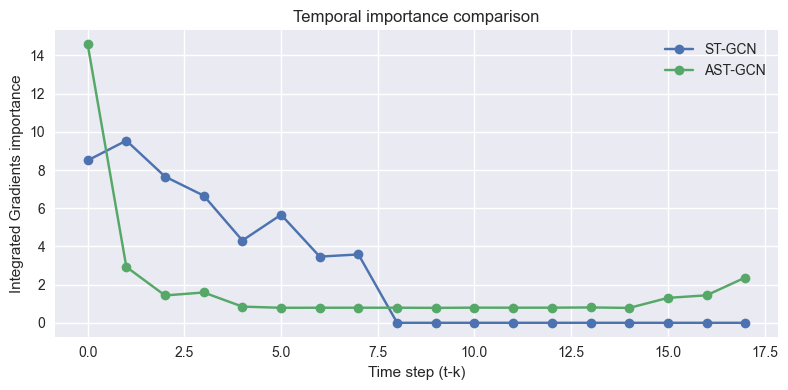
\includegraphics[width=0.92\linewidth]{figures/temporal_importance_comparison.png}
    \caption{Integrated Gradients temporal attribution}
    \label{fig:app_ig_temporal}
\end{figure}

The POI feature-level attribution figure is exported from the notebook plot titled \textbf{``POI feature-level attribution (POI ST-GCN)''} and saved as \texttt{figures/poi\_feature\_attribution.png}.

\begin{figure}[!htbp]
    \centering
    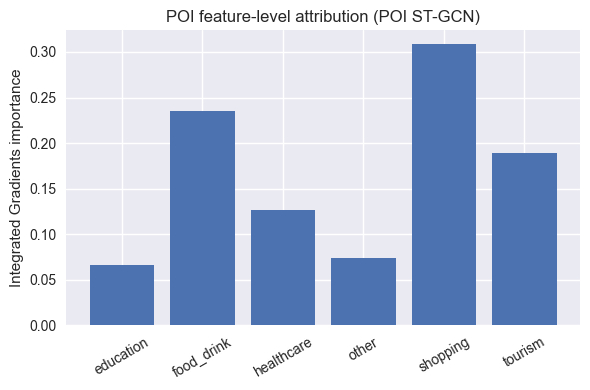
\includegraphics[width=0.78\linewidth]{figures/poi_feature_attribution.png}
    \caption{Integrated Gradients over POI categories}
    \label{fig:app_ig_poi}
\end{figure}

\section{PGExplainer-style edge influence example}
A mask-based explainer inspired by PGExplainer is used to rank influential edges for a target station \cite{luo2020pgexplainer}. The table below reproduces the notebook’s printed top incoming edges for \texttt{station\_id=1}.

\begin{table}[!htbp]
\centering
\small
\caption{Top incoming edges for target station \texttt{station\_id=1} from the notebook’s mask-based edge explanation (PGExplainer-style).}
\label{tab:app_pgexplainer_edges}
\renewcommand{\arraystretch}{1.15}
\begin{tabular}{ccc}
\hline
\textbf{Rank} & \textbf{Edge (from $\rightarrow$ to)} & \textbf{Weight} \\
\hline
1  & 14 $\rightarrow$ 1 & 0.9064 \\
2  & 10 $\rightarrow$ 1 & 0.8984 \\
3  & 9  $\rightarrow$ 1 & 0.8965 \\
4  & 27 $\rightarrow$ 1 & 0.8838 \\
5  & 98 $\rightarrow$ 1 & 0.8799 \\
6  & 52 $\rightarrow$ 1 & 0.8479 \\
7  & 37 $\rightarrow$ 1 & 0.8016 \\
8  & 71 $\rightarrow$ 1 & 0.0948 \\
9  & 53 $\rightarrow$ 1 & 0.0937 \\
10 & 17 $\rightarrow$ 1 & 0.0862 \\
\hline
\end{tabular}
\end{table}

\section{Supplementary station-level performance visuals}
The following figures are included for additional context and are exported directly from notebook plots.

\begin{figure}[!htbp]
    \centering
    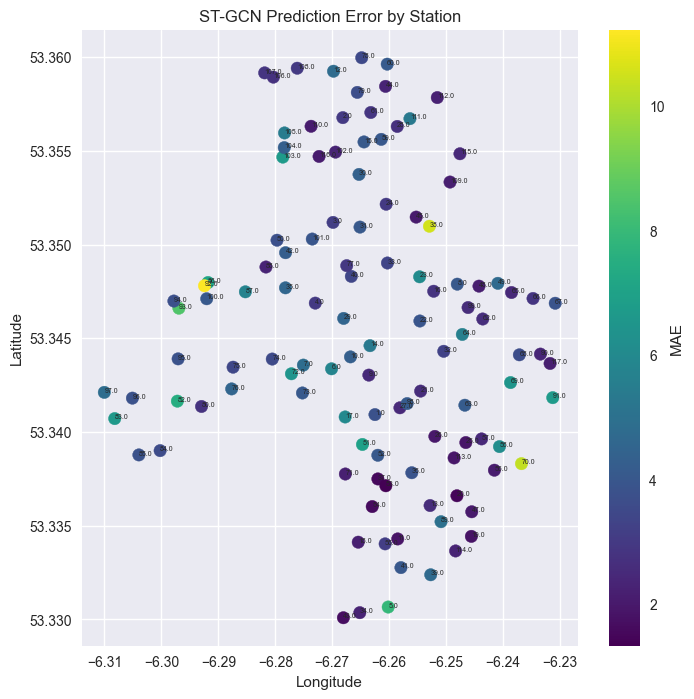
\includegraphics[width=0.92\linewidth]{figures/stgcn_error_by_station.png}
    \caption{Station-level MAE visualization}
    \label{fig:app_stgcn_error_station}
\end{figure}

\begin{figure}[!htbp]
    \centering
    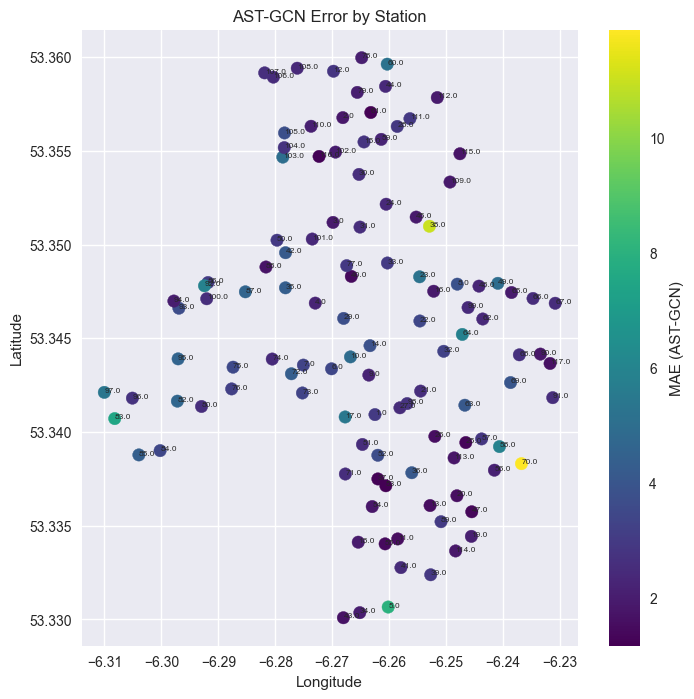
\includegraphics[width=0.92\linewidth]{figures/astgcn_error_by_station.png}
    \caption{Station-level MAE visualization}
    \label{fig:app_astgcn_error_station}
\end{figure}

\begin{figure}[!htbp]
    \centering
    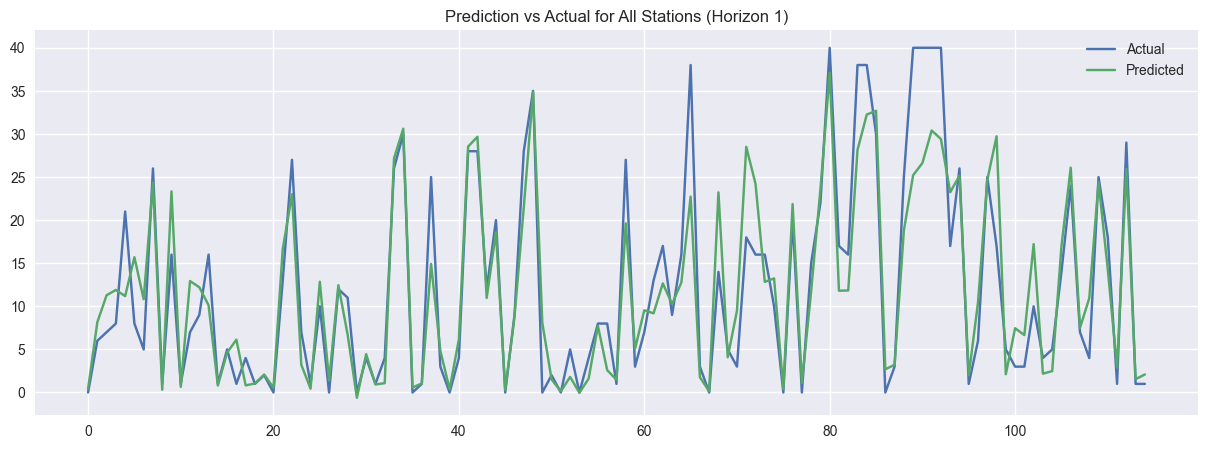
\includegraphics[width=0.92\linewidth]{figures/pred_vs_actual_h1.png}
    \caption{Forecast sanity-check plot}
    \label{fig:app_pred_vs_actual_h1}
\end{figure}


\end{document}